\begin{center}
\noindent \textbf{\underbar{``MODELO DIMENSIONAL VS MODELO TABULAR''}}
\end{center}

\begin{enumerate}
\item  \textbf{MARCO TEORICO}
\end{enumerate}

\noindent \textbf{\underbar{MODELO DIMENSIONAL}}

\noindent \textbf{\underbar{}}

\noindent B\'{a}sicamente el Modelo Dimensional es el nombre que se le da a una t\'{e}cnica utilizada especialmente en Data Warehouses. Este modelo difiere bastante del modelo Entidad-Relaci\'{o}n que normalmente conocemos.

\noindent 

\noindent El Modelo Dimensional busca presentar la informaci\'{o}n de una manera est\'{a}ndar, sencilla y sobre todo intuitiva para los usuarios, adem\'{a}s de que permite accesos a la informaci\'{o}n mucho m\'{a}s r\'{a}pida por parte de los manejadores de bases de datos.

\noindent 

\noindent Cada Modelo Dimensional est\'{a} compuesto por una tabla llamada ``de hechos'' y por un conjunto de peque\~{n}as tablas llamadas ``dimensiones ``. Cada dimensi\'{o}n contiene una llave primaria que se ``conecta'' a la tabla de hechos manteniendo una relaci\'{o}n de 1 a muchos).
\begin{center}
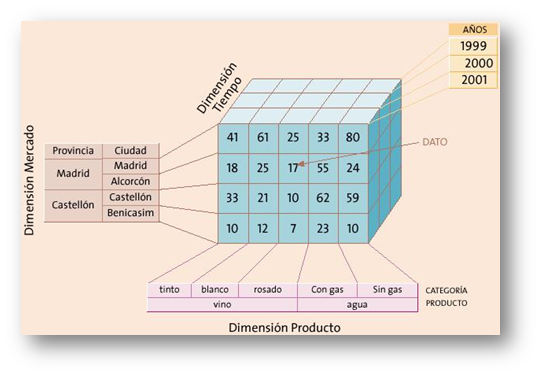
\includegraphics[width=7cm, height=5cm]{Imagenes/modelo_dimensional}
\end{center}
\begin{enumerate}
\item  \textbf{Modelo dimensional}

\end{enumerate}

\noindent 

\begin{enumerate}
\item  Define un nivel mínimo de detalle
(granularidad)

\item  Se compone de:

  - Hechos \\
  - Medidas\\
  - Dimensiones\\
  - Atributos\\
        Elementos\\
        Jerarquías\\
  - Relaciones\\

\begin{center}
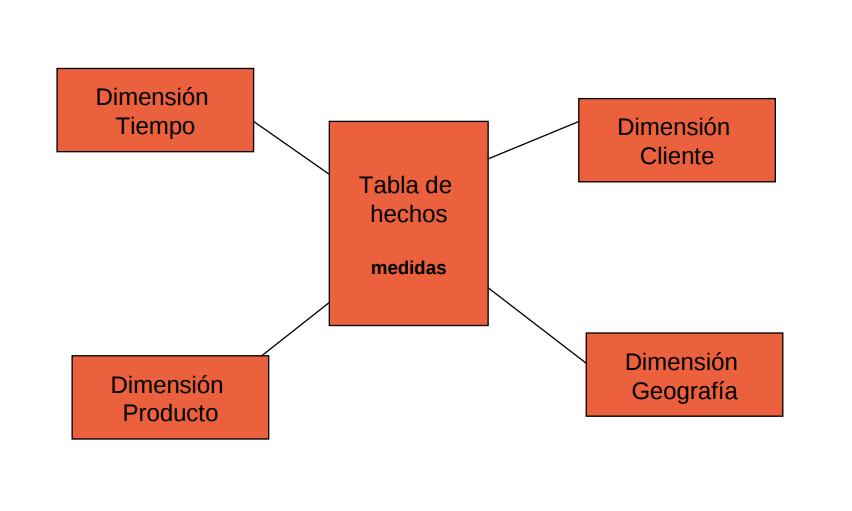
\includegraphics[width=7cm, height=5cm]{Imagenes/modelo_dimensional1}
\end{center}
\end{enumerate}

\noindent 

\begin{enumerate}
\item  \textbf{Modelo dimensional o multidimensional}
\end{enumerate}

\noindent \textbf{}
\noindent El modelo multidimensional dentro del entorno de las bases de datos es una disciplina de dise\~{n}o que se sustenta en el modelo entidad-relaci\'{o}n y en las realidades de la ingenier\'{i}a de texto y datos num\'{e}ricos. 

\noindent 

\noindent Modela las particularidades de los procesos que ocurren en una organizaci\'{o}n, dividi\'{e}ndolos en mediciones y entorno. Las medidas son en su mayor\'{i}a, medidas num\'{e}ricas, y se les denomina hechos. Alrededor de estos hechos existe un contexto que describe en qu\'{e} condiciones y en qu\'{e} momento se registr\'{o} este hecho. Aunque el entorno se ve como un todo, existen registros l\'{o}gicos de diferentes caracter\'{i}sticas que describen un hecho, por ejemplo, si el hecho referido, es la venta de un producto en una cadena de tiendas, se podr\'{i}a dividir el entorno que rodea al hecho de la cantidad vendida, en el producto vendido, el cliente que lo compr\'{o}, la tienda y la fecha en que se realiz\'{o} la venta. A estas divisiones se le denomina dimensiones y a diferencia de los hechos que son num\'{e}ricos, estos son fundamentalmente textos descriptivos.

\noindent 

\noindent Las medidas, como se expres\'{o} anteriormente, se registran en las tablas de hechos, siendo la llave de esta tabla, la combinaci\'{o}n de las m\'{u}ltiples llaves for\'{a}neas que hacen referencia   a las dimensiones que describen la ocurrencia de este hecho, en otras palabras, cada una de las llaves extranjeras en las tablas de hecho se corresponden con la llave primaria de una dimensi\'{o}n. 


\noindent 

\begin{enumerate}
\item  \textbf{Proceso de negocio}
\end{enumerate}

\noindent 


\noindent Un proceso de negocio es un conjunto de tareas relacionadas l\'{o}gicamente llevadas a cabo para lograr un resultado de negocio definido. Cada proceso de negocio tiene sus entradas, funciones y salidas. Las entradas son requisitos que deben tenerse antes de que una funci\'{o}n pueda ser aplicada. Cuando una funci\'{o}n es aplicada a las entradas de un m\'{e}todo, tendremos ciertas salidas resultantes.

\noindent 

\noindent Es una colecci\'{o}n de actividades estructurales relacionadas que producen un valor para la organizaci\'{o}n, sus inversores o sus clientes. Es, por ejemplo, el proceso a trav\'{e}s del que una organizaci\'{o}n ofrece sus servicios a sus clientes.

\noindent 

\noindent Un proceso de negocio puede ser parte de un proceso mayor que lo abarque o bien puede incluir otros procesos de negocio que deban ser incluidos en su funci\'{o}n. En este contexto un proceso de negocio puede ser visto a varios niveles de granularidad. El enlace entre procesos de negocio y generaci\'{o}n de valor lleva a algunos practicantes a ver los procesos de negocio como los flujos de trabajo que efect\'{u}an las tareas de una organizaci\'{o}n. 

\noindent 

\noindent Los procesos poseen las siguientes caracter\'{i}sticas:

\noindent 

\begin{enumerate}
\item  Pueden ser medidos y est\'{a}n orientados al rendimiento

\item  Tienen resultados espec\'{i}ficos

\item  Entregan resultados a clientes o ``stakeholders''

\item  Responden a alguna acci\'{o}n o evento espec\'{i}fico

\item  Las actividades deben agregar valor a las entradas del proceso.
\end{enumerate}

\noindent 

\noindent Los procesos de negocio pueden ser vistos como un recetario para hacer funcionar un negocio y alcanzar las metas definidas en la estrategia de negocio de la empresa. Las dos formas principales de visualizar una organizaci\'{o}n son la vista funcional y la vista de procesos.

\noindent 

\noindent Hay tres tipos de procesos de negocio:

\noindent 

\begin{enumerate}
\item  Procesos estrat\'{e}gicos -- Estos procesos dan orientaci\'{o}n al negocio. Por ejemplo, ``Planeacion estrategica'', ``Establecer objetivos y metas''.

\item  Procesos sustantivos-- Estos procesos dan el valor al cliente, son la parte principal del negocio. Por ejemplo, ``Repartir mercanc\'{i}as''.

\item  \includegraphics*[width=4.21in, height=2.54in, keepaspectratio=false]{image5}Procesos de apoyo vertical u horizontal -- Estos procesos dan soporte a los procesos centrales. Por ejemplo, ``Registrar los hechos econ\'{o}micos'', ``Dar Soporte/Servicio t\'{e}cnico''.
\end{enumerate}

\noindent 
\noindent 
\noindent 



\noindent \textbf{\underbar{MODELO TABULAR}}

\noindent \textbf{\underbar{}}

\noindent En t\'{e}rminos muy simples un modelo tabular es una base de datos OLAP cuyo almacenamiento est\'{a} en memoria RAM. Debido a su enfoque (similar a una base de datos columnar) alcanza altos ratios de compresi\'{o}n gestionando gran cantidad de informaci\'{o}n en poca memoria. Debido a que est\'{a} en memoria ofrece un r\'{a}pido acceso a la informaci\'{o}n.

\noindent 


\begin{enumerate}
\item  \textbf{Ventajas}
\end{enumerate}

\noindent Al implementar un modelo tabular se crea una base de datos del modelo en un entorno de pruebas, ensayo o producci\'{o}n. Los usuarios pueden conectarse al modelo implementado mediante un archivo de conexi\'{o}n. bism en Sharepoint o mediante una conexi\'{o}n de datos directamente desde las aplicaciones cliente de informes, como Microsoft Excel, Power View, o una aplicaci\'{o}n personalizada. La base de datos del \'{a}rea de trabajo del modelo, que se genera al crear un proyecto de modelo tabular en SQL Server Data Tools (SSDT)y se usa para crear el modelo, permanecer\'{a} en la instancia del servidor del \'{a}rea de trabajo, lo que permite realizar cambios en el proyecto de modelo y volver a implementarlo despu\'{e}s en el entorno de pruebas, ensayo o producci\'{o}n cuando sea necesario.

\noindent 


\begin{enumerate}
\item  \textbf{Implementar un modelo tabular de SQL Server Data Tools (SSDT)}
\end{enumerate}

\noindent \textbf{}

\noindent La implementaci\'{o}n es un proceso sencillo; sin embargo, se deben realizar algunos pasos para asegurarse de que el modelo se implementa en la instancia adecuada de Analysis Services y con las opciones de configuraci\'{o}n correctas.

\noindent 

\noindent Los modelos tabulares se definen con varias propiedades espec\'{i}ficas de la implementaci\'{o}n. Durante la implementaci\'{o}n, se establece una conexi\'{o}n con la instancia de Analysis Services especificada en la propiedad Servidor. 

\noindent 

\begin{center}
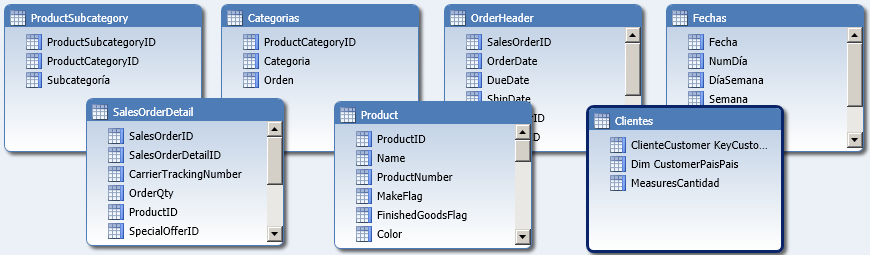
\includegraphics[width=7cm, height=5cm]{Imagenes/modelo_tabular}
\end{center}



\begin{enumerate}
\item  \textbf{Modelo tabular vs Modelo dimensional }
\end{enumerate}



\begin{center}
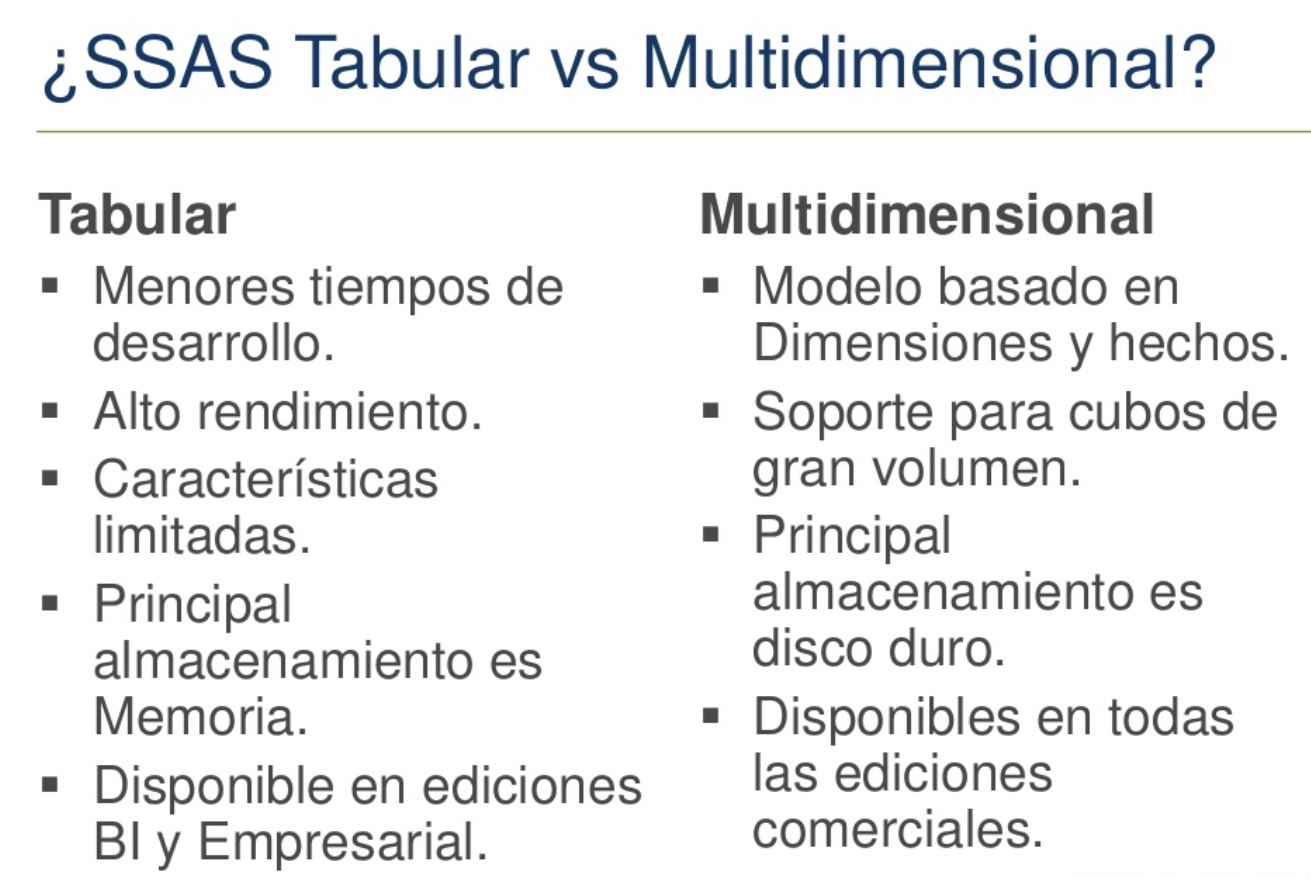
\includegraphics[width=15cm, height=10cm]{Imagenes/modelo_tabular_vs_dimensional}
\end{center}


\section{CONCLUSIONES}
\begin{enumerate}
\item  A partir del estudio de los modelos multidimensional y tabular, la experiencia adquirida en el desarrollo del sistema y el comportamiento de los resultados obtenidos en los experimentos llevados a cabo, se pudo realizar una comparaci\'{o}n cualitativa y pr\'{a}ctica de ambas opciones. Como resultado, se esbozaron consideraciones generales en cuanto a fortalezas y debilidades contribuyendo al trabajo ulterior en esta \'{a}rea del conocimiento. Se concluye que el modelo tabular ofrece una alternativa de modelaci\'{o}n con la que los usuarios se identifican mejor a partir de sus necesidades de an\'{a}lisis y consultas, pero se basa en el uso y el aprovechamiento de elevados recursos de hardware, principalmente memoria RAM. Por otro lado, se corrobor\'{o} que el modelo multidimensional puede constituir la mejor opci\'{o}n si se requiere una compleja modelaci\'{o}n de la l\'{o}gica del negocio o se necesita una soluci\'{o}n escalable y que maneje grandes vol\'{u}menes de datos.

\item  El modelo dimensional y el novedoso modelo tabular, as\'{i} como en las funcionalidades de herramientas de visualizaci\'{o}n como Microsoft Excel y Power View, en funci\'{o}n de agilizar y enriquecer el ambiente anal\'{i}tico puesto a disposici\'{o}n de los especialistas y ejecutivos. Se constat\'{o} que el modelo tabular no constituye un aporte conceptualmente diferente, sino una implementaci\'{o}n alternativa del modelo dimensional de datos para la herramienta de procesamiento anal\'{i}tico SQL Server 2012 Analysis Services, aun cuando el soporte sobre el almacenamiento columnar y las bases de datos in-memory le aportan un inter\'{e}s actual y una perspectiva fruct\'{i}fera al modelo tabular, m\'{a}s all\'{a} de lo que puede ofrecer Microsoft.
\end{enumerate}










